\documentclass[aspectratio=43,10pt]{beamer}

% ==================================================
% PREAMBLE
% ==================================================

% Theme
\usetheme{default}
\usecolortheme{default}

% Packages
\usepackage{amsmath}
\usepackage{booktabs}
\usepackage{listings}
\usepackage{xcolor}

\usepackage{tikz,pgfplots}
\pgfplotsset{compat=1.18}

% Colors
\definecolor{priorblue}{RGB}{49,95,160}
\definecolor{datagreen}{RGB}{36,130,90}
\definecolor{postred}{RGB}{180,65,55}
\definecolor{aggiemaroon}{RGB}{80,0,0}
\definecolor{gold}{RGB}{200,155,60}
\definecolor{lightgold}{RGB}{248,240,220}

% Beamer settings
\setbeamertemplate{navigation symbols}{}
\setbeamertemplate{footline}[frame number]

\setbeamercolor{structure}{fg=aggiemaroon}
\setbeamercolor{frametitle}{fg=aggiemaroon}

\setbeamerfont{frametitle}{series=\bfseries}
\setbeamerfont{normal text}{size=\small}

% Commands
\newcommand{\CFP}{C_{\mathrm{FP}}}
\newcommand{\CFN}{C_{\mathrm{FN}}}
\newcommand{\Risk}{\mathcal{R}}
\newcommand{\answer}[1]{\textcolor{red}{#1}}

%\newtcolorbox{atencao}{colback=lightgold,colframe=gold,boxrule=0.7pt}

% Title information
\title{Decision and Risk Analysis}
\subtitle{Decision Rule Problems}
\author{\emph{}}

\date{
  \color{aggiemaroon}{
    DAEN 427 / ISEN 427 / ISEN 627\\
    \textbf{Alexander Abuabara}\\
    Fall 2026
  }
}

\titlegraphic{
  \vfill
  
\includegraphics[height=1.2cm]{TAMU_logo.png}
}

% ==================================================
% DOCUMENT
% ==================================================

\begin{document}

% ==================================================
% TITLE SLIDE
% ==================================================

\maketitle

% ==================================================
% DECISION RULE
% ==================================================

\begin{frame}{Formulas}

  \begin{columns}[T,onlytextwidth]

    \column{0.47\textwidth}

    \begin{block}{Probability model}

      The prior and data produce the probability to the decision:

      \[
      q=P(H=1\mid D).
      \]

      For a next case, $q$ may be posterior predictive.

      For a process claim, $q$ may be a posterior tail probability.

    \end{block}

    \column{0.49\textwidth}

    \begin{block}{Loss model}

      With zero loss for correct decisions,

      \[
      \Risk(a_+)=\CFP(1-q),
      \]

      \[
      \Risk(a_-)=\CFN q.
      \]

      Take the positive action when

      \[
      q>\tau,
      \qquad
      \tau=\frac{\CFP}{\CFP+\CFN},
      \]

      \[
      \tau=\frac{1}{1+r},
      \]

      where $r=\CFN/\CFP$.

    \end{block}

  \end{columns}

\end{frame}

% ==================================================
% SUMMARY
% ==================================================

\begin{frame}{Formulas}

  \begin{columns}[T,onlytextwidth]

    \column{0.48\textwidth}

    \begin{block}{Question 1: next case}

      Decision target:

      \[
      Y_{\mathrm{new}}=1.
      \]

      Probability:

      \[
      P(Y_{\mathrm{new}}=1\mid D)
      =E(\theta\mid D).
      \]

    \end{block}

    \column{0.48\textwidth}

    \begin{block}{Question 2: process state}

      Decision target:

      \[
      \theta>\theta_0.
      \]

      Probability:

      \[
      P(\theta>\theta_0\mid D).
      \]
      
    \end{block}

  \end{columns}

\end{frame}

% ==================================================
% QUESTION 1
% ==================================================

\begin{frame}{Q1) Screening a transaction for fraud}

  An online retailer models the fraud probability $\theta$ for
  transactions in a new risk segment. Before observing segment data,

  \[
  \theta\sim\operatorname{Beta}(2,18).
  \]

  Among the first 24 transactions, 6 were fraudulent. For the next
  transaction, the retailer may send it to manual review ($a_+$) or
  approve it automatically ($a_-$).

  \vspace{0.15cm}

  \begin{enumerate}
    \item[a.] Find the posterior distribution of $\theta$.

    \item[b.] Find the posterior predictive probability that the next
          transaction is fraudulent.

    \item[c.] If $\CFP=\$25$ and $\CFN=\$180$, find the action threshold
          and the Bayes action. Verify the decision using expected losses.

    \item[d.] Find the critical false-negative cost above which manual review
          becomes optimal, holding $\CFP=\$25$ fixed.
  \end{enumerate}

\end{frame}

% ==================================================
% Q1a
% ==================================================

\begin{frame}{}
\begin{block}{Q1a ... posterior distribution}
  \textbf{Step 1.} Identify the prior parameters and observed counts:

  \[
  \alpha=2,\quad \beta=18,\quad y=6,\quad n-y=18.
  \]
  
  \pause

  \textbf{Step 2.} Apply Beta--Binomial conjugacy:

  \[
  \theta\mid D\sim
  \operatorname{Beta}(\alpha+y,\,\beta+n-y).
  \]

  \pause
  
  \textbf{Step 3.} Substitute the values:

  \[
  \theta\mid D\sim
  \operatorname{Beta}(2+6,\,18+18).
  \]

  \textcolor{blue}{Answer:}

  \answer{
    $\theta \mid D\sim\operatorname{Beta}(8,36)$
    The six observed frauds increase the prior fraud count from 2 to 8.
  }
\end{block}
\end{frame}

% ==================================================
% Q1b
% ==================================================

\begin{frame}{}
\begin{block}{Q1b ... probability for the next transaction}

  The decision concerns one future binary outcome, so use the
  Beta--Bernoulli posterior predictive probability.

  \[
  Y_{\mathrm{new}} =
  \begin{cases}
    1, & \text{if the next transaction is fraudulent},\\
    0, & \text{if the next transaction is legitimate}.
  \end{cases}
  \]

  and $D$ represents all the observed data used to update the prior
  distribution.
  
  \pause

  \textbf{Step 1.} Use the posterior mean:

  \[
  q=P(Y_{\mathrm{new}}=1\mid D)=E(\theta\mid D).
  \]
  
  \pause

  \textbf{Step 2.} Insert the posterior parameters:

  \[
  q=\frac{8}{8+36}=\frac{8}{44}=\frac{2}{11}.
  \]

  \textcolor{blue}{Answer:}

  \answer{
    $q\approx0.1818$.
    The model assigns an 18.18\% fraud probability to the next
    transaction in this segment.
  }

\end{block}
\end{frame}

% ==================================================
% Q1c
% ==================================================

\begin{frame}{}
\begin{block}{Q1c ... loss table}
  \small

  \[
  \begin{array}{c|cc}
    \toprule
    \textbf{Decision}
    &
    \textbf{Fraudulent }(Y_{\mathrm{new}}=1)
    &
    \textbf{Legitimate }(Y_{\mathrm{new}}=0)
    \\
    \midrule
    \text{Manual review }(a_+)
    &
    \text{Correct positive: } \$0
    &
    \text{False positive: } \$25
    \\[4pt]
    \text{Automatic approval }(a_-)
    &
    \text{False negative: } \$180
    &
    \text{Correct negative: } \$0
    \\
    \bottomrule
  \end{array}
  \]
\end{block}
\end{frame}

% ==================================================
% Q1c
% ==================================================

\begin{frame}{}
\begin{block}{Q1c ... threshold and Bayes action}
  \textbf{Step 1.} Convert costs to an action threshold:

  \[
  \tau=\frac{25}{25+180}=\frac{5}{41}\approx0.1220.
  \]
  
  \pause

  \textbf{Step 2.} Compare probability with threshold:

  \[
  q=0.1818>0.1220=\tau.
  \]

  Manual review has the smaller posterior expected loss.
  
  \pause

  \textbf{Step 3.} Verify directly:

  \[
  \Risk(a_+)=25(1-2/11)=\$20.45,
  \]

  \[
  \Risk(a_-)=180(2/11)=\$32.73.
  \]

  \textcolor{blue}{Answer:}
  \answer{Send the next transaction to manual review.}
\end{block}
\end{frame}

% ==================================================
% Q1d
% ==================================================

\begin{frame}{}
\begin{block}{Q1d ... critical false-negative cost}
  Manual review becomes optimal when

  \[
  \CFP(1-q)<\CFN q.
  \]
  
  \pause

  \textbf{Step 1.} Solve for $\CFN$:

  \[
  \CFN>\CFP\frac{1-q}{q}.
  \]
  
  \pause
  
  \textbf{Step 2.} Substitute $\CFP=25$ and $q=2/11$:

  \[
  \CFN>25\frac{9/11}{2/11}
  =25\left(\frac{9}{2}\right)
  =112.50.
  \]

  \textcolor{blue}{Answer:}

  \answer{
    Manual review is optimal when $\CFN>\$112.50$.\\
    At $\CFN=\$112.50$, the retailer is indifferent.\\
    The stated cost of $\$180$ lies above the boundary.
  }
\end{block}
\end{frame}

% ==================================================
% QUESTION 2
% ==================================================

\begin{frame}{Q2) Intervening in a production process}

  A food plant tracks the contamination rate $\theta$ for a production
  line. The prior is
  \[
  \theta\sim\operatorname{Beta}(2,8).
  \]

  Testing finds 8 contaminated samples among 20. Management defines the
  adverse state as $H=1$ when $\theta>0.25$. It may stop and sanitize the
  line ($a_+$) or continue production ($a_-$).

  \vspace{0.1cm}

  \begin{enumerate}
    \item[a.] Find the posterior distribution of $\theta$.

    \item[b.] Compute $q=P(\theta>0.25\mid D)$.\\
    		  {
		      \tiny
              Note, from R:
              \textcolor{blue}{\texttt{> pbeta(0.25, shape1 = 10, shape2 = 20, lower.tail = TRUE)}}
              $\rightarrow$ \textcolor{red}{\texttt{[1] 0.1663049}}
              }

    \item[c.] With $\CFP=\$40{,}000$ and $\CFN=\$120{,}000$, find the
          threshold, choose the Bayes action, and compare expected losses.

    \item[d.] If the scientific threshold changes from $0.25$ to $0.35$,
          recompute $q$ and determine whether the action changes. Find the
          critical cost ratio for this revised state.\\
    		  {
		      \tiny
              Note, from R:
              \textcolor{blue}{\texttt{> 1 - pbeta(0.35, shape1 = 10, shape2 = 20, lower.tail = TRUE)}}
              $\rightarrow$ \textcolor{red}{\texttt{[1] 0.4076133}}
              }
  \end{enumerate}

\end{frame}

% ==================================================
% Q2a
% ==================================================

\begin{frame}{}
\begin{block}{Q2a ... posterior distribution}
  \textbf{Step 1.} Record the counts:

  \[
  \alpha=2,\quad \beta=8,\quad y=8,\quad n-y=12.
  \]
  
  \pause

  \textbf{Step 2.} Update both Beta parameters:

  \[
  \theta\mid D\sim
  \operatorname{Beta}(\alpha+y,\,\beta+n-y).
  \]
  
  \pause

  \textbf{Step 3.} Substitute:

  \[
  \theta\mid D\sim
  \operatorname{Beta}(2+8,\,8+12).
  \]

  \textcolor{blue}{Answer:}

  \answer{
    $\theta\mid D\sim\operatorname{Beta}(10,20)$.\\
    Its posterior mean is $10/30=0.3333$.\\
    But the decision requires a tail probability rather than the mean.
  }
\end{block}
\end{frame}

% ==================================================
% Q2b
% ==================================================

\begin{frame}{}
\begin{block}{Q2b ... probability of an excessive rate}

The posterior mean of $0.3333$ does not directly answer the question of how
likely $\theta$ is to be greater than $0.25$.

To answer that question, we must consider the entire posterior distribution.

\pause

Because $\theta$ is unknown, we calculate
\[
q=P(\theta>0.25\mid D).
\]
This is the probability that the true contamination rate is greater than 25\%,
given the observed data.
\end{block}
\end{frame}

\begin{frame}{}
\begin{block}{Q2b ... probability of an excessive rate}
\begin{figure}[ht]
\centering
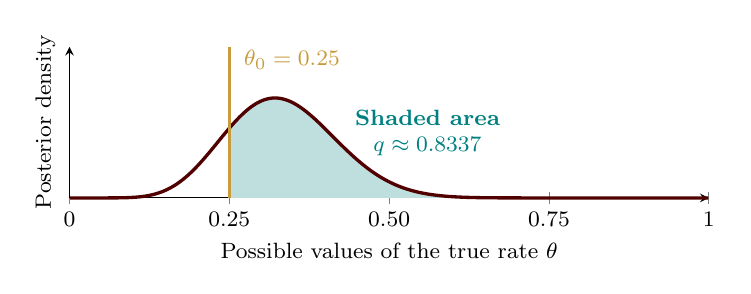
\begin{tikzpicture}
\footnotesize
\begin{axis}[
  width=0.80\textwidth,
  height=3.5cm,
  xmin=0, xmax=1, ymin=0,
  axis lines=left,
  xlabel={Possible values of the true rate $\theta$},
  ylabel={Posterior density},
  xtick={0,0.25,0.5,0.75,1},
  xticklabels={$0$,$0.25$,$0.50$,$0.75$,$1$},
  ytick=\empty,
  samples=250,
  domain=0.001:0.999,
  clip=false
]
\addplot[draw=none,fill=teal!25,domain=0.25:0.999]
  {200300100*x^9*(1-x)^19} \closedcycle;
\addplot[very thick,aggiemaroon,domain=0.001:0.999]
  {200300100*x^9*(1-x)^19};
\addplot[very thick,gold] coordinates {(0.25,0) (0.25,7)};
\node[anchor=west,text=gold,font=\bfseries]
  at (axis cs:0.26,6.4) {$\theta_0=0.25$};
\node[align=center,text=teal,font=\bfseries]
  at (axis cs:0.56,3.0) {Shaded area\\$q\approx0.8337$};
\end{axis}
\end{tikzpicture}
\caption{\footnotesize Posterior $\operatorname{Beta}(10,20)$ distribution. Shaded
area represents $P(\theta>0.25\mid D)$.}
\end{figure}

The shaded area is $q=P(\theta>0.25\mid D)\approx0.8337.$

Given the model, the prior, and the test results, we assign an 83.37\%
posterior probability to the claim that the true contamination rate exceeds
25\%.

\end{block}
\end{frame}

\begin{frame}{}
\begin{block}{Q2b ... probability of an excessive rate}
  The state concerns the underlying rate, so calculate a posterior tail
  probability.
  
  \textbf{Step 1.} Define the relevant probability:

  \[
  q=P(\theta>0.25\mid D).
  \]
  
  \textbf{Step 2.} Use the Beta posterior CDF:

  \[
  q=1-F_{\operatorname{Beta}(10,20)}(0.25).
  \]
    
  \textbf{Step 3.} Evaluate the CDF numerically:

  \[
  q\approx1-0.166305=0.833695.
  \]

  \textcolor{blue}{Answer:}

  \answer{
    $P(\theta>0.25\mid D)\approx0.8337$.\\
    The posterior assigns an 83.37\% probability to the adverse process
    state.
  }
\end{block}
\end{frame}

% ==================================================
% Q2c
% ==================================================

\begin{frame}{}
\begin{block}{Q2c ... intervention decision}
  \textbf{Step 1.} Convert the costs to a threshold:

  \[
  \tau=\frac{40{,}000}{40{,}000+120{,}000}=0.25.
  \]
  
  \pause

  \textbf{Step 2.} Compare $q$ and $\tau$:

  \[
  0.8337>0.25.
  \]
  
  \pause

  \textbf{Step 3.} Compare expected losses in thousands of dollars:

  \[
  \Risk(a_+)=40(1-0.833695)\approx6.65,
  \]

  \[
  \Risk(a_-)=120(0.833695)\approx100.04.
  \]

  \textcolor{blue}{Answer:}

  \answer{Stop and sanitize the production line.}
\end{block}
\end{frame}

% ==================================================
% Q2d
% ==================================================

\begin{frame}{}
\begin{block}{Q2d ... revised state threshold}
  Management now defines the adverse state as $\theta>0.35$. The costs
  do not change.

  \textbf{Step 1.} Recompute the state probability:

  \[
  q_{0.35}=1-F_{\operatorname{Beta}(10,20)}(0.35)
  \approx0.4076.
  \]
  
  \pause

  \textbf{Step 2.} Compare with the unchanged action threshold:

  \[
  0.4076>0.25=\tau.
  \]

  The Bayes action remains to stop and sanitize.
  
  \pause

  \textbf{Step 3.} Find the critical cost ratio:

  \[
  r_{\mathrm{crit}}=\frac{1-q_{0.35}}{q_{0.35}}
  =\frac{0.5924}{0.4076}\approx1.453.
  \]

  \textcolor{blue}{Answer:}

  \answer{
    The action remains positive because the actual ratio $r=120/40=3$
    exceeds $r_{\mathrm{crit}}\approx1.453$.
  }
\end{block}
\end{frame}

% ==================================================
% END
% ==================================================

\end{document}